
% SEP 2012 Group 13
% Software Requirements Document (SRS)
%
\documentclass[11pt, a4paper]{report}
\usepackage{graphicx}
\usepackage{fullpage}
\usepackage{url}
\pagestyle{headings}

%%% page parameters
\headsep = 25pt
\begin{document}
\oddsidemargin -0.5 cm
\evensidemargin -0.5 cm
\textwidth 15 cm
\topmargin -1.2 cm
\textheight 25 cm
\begin{center}

\includegraphics[scale=1.5]{./UniLogo}\\[1cm]    
\textbf{\Huge \bfseries User Manual}\\[1.5cm]
\textbf{\huge for}\\[0.5cm]


% Title
\textbf{ \huge Archaeology Robot }\\[0.3cm]
\textbf{ \huge Team 13 }\\[2cm]


\begin{tabular}{ |c | p{2cm} |}
	\hline
Yufeng Bai 1600095 & \\[.5cm] \hline
Jun Chen 1206265 & \\[.5cm] \hline
Dawei Geng 1219181 & \\[.5cm] \hline
Yunyao Yao 1203525 & \\[.5cm] \hline
Shikai Li 1214223 & \\[.5cm] \hline
Quang Khoi Nguyen 1187070  & \\[.5cm] \hline
Yatong Zhou 1204471 & \\[.5cm] \hline
\end{tabular}


\vfill

% Bottom of the page
Version 1.0 \\ [0.2cm]
{\large \today}

\end{center}


\tableofcontents



% Version History %

% IMPORTANT %
% Whenever you make a change to this document you MUST put an entry in below
% Must conform to firstName lastName &  date & discription \\ \hline


\clearpage
\section*{Revision History}
\begin{tabular}{| l | l | l | l | }
\hline
Name      		&	Date        	&	Reason For Changes                  	  	&	Version     	\\ \hline
Dawei Geng      & 	21 Aug 2012    	& 	basic framework of the SPMP and Chapter 1 	&	0.1             \\ \hline
Dawei Geng      & 	23 Aug 2012    	& 	Chapter 3 \& Section 4.1 				    &	0.19			\\ \hline
Dawei Geng      &	24 Aug 2012     &	Section 4.2.1 \& 4.2.2                 		&	0.2 	     	\\ \hline
Dawei Geng     	&	25 Aug 2012     &	Chapter 5                  	  				&	0.3		    	\\ \hline
Jun Chen      	   &	25 Aug 2012        	&	Spelling and grammar check , error fix               	  	&	0.31     	\\ \hline
%Name      		&	Date        	&	Reason For Changes                  	  	&	Version     	\\ \hline
%Name      		&	Date        	&	Reason For Changes                  	  	&	Version     	\\ \hline
%Name      		&	Date        	&	Reason For Changes                  	  	&	Version     	\\ \hline






\end{tabular}
\clearpage

% Introduction %

\chapter{Introduction}

\section{Purpose and Scope}
This document is aim to provide information that are required to manage the overall design, implementation, maintenance of the project of archaeology robot. 

This document will be divided in to seven parts, including the Introduction, Definitions, Project organization, Risk management plan, Process model, Work plan, and the Supporting plans.

\begin{enumerate}
	\item \textbf{Project organization} describes the responsibilities for each member of the team and the reason behind this arrangement.
	\item \textbf{Risk management} outlines the risks may be found during the development of the project, also includes risk analysis and the processes and strategies for the team members to control or overcome these risks.
	\item \textbf{Process model} describes the process model will be used throughout the whole development. Including the critical paths and major stages taken in the development. Rational behind this choice will be provided, along with the advantages and disadvantages of this process model. 
	\item \textbf{Work plan} includes the tasks will be done to deliver the product, and the milestones that the team will be meeting during the development. Work plan will also includes the duration of the tasks and the allocation of the resources to these tasks.
	\item \textbf{Supporting plan} outlines the configuration management plan, the documentation plan, and quality assurance plan.
\end{enumerate}


\section{Assumptions and constraints}
This project will be developed under such assumptions and constraints:
\begin{enumerate}
	\item All the team members will have a computer which is installed LejOS.
	\item All the team members' PC will have a JAVA RE and SDK.
	\item All the team members will have access to the group's SVN repository.
	\item A Bluetooth connection can be created between the robot and every team member's PC.
	\item A Lego Mindstorm NXT robot will be used in this project. 
	\item This project has a duration of 11 weeks.
	\item This project will require at least 10 hours per week workload for each team member.
\end{enumerate}

\section{Project deliverables}
The following items will be delivered to the client throughout the development of this project.
\begin{enumerate}
	\item Team Poster
	\item Software Requirement Specification (SRS)
	\item Software Project Management Plan (SPMP)
	\item Software Design Document (SDD)
	\item Testing Report
	\item User Manual
	\item Project Milestone Demonstration
	\item Final Project Demonstration
\end{enumerate}


\section{Evolution of the plan}
This plan will be made by the team during the requirements elicitation and system design. The plan shall be made by gathering the feedback from the clients, and negotiation with clients about the milestones. In the software developing stage, the plan shall be changed under such circumstances:
\begin{enumerate}
	\item Requirements changed by the clients
	\item A defect of the plan was found
	\item Other unexpected situations
\end{enumerate}

At the planning stage, clients shall be able to change or raise requirements at anytime. However once the plan have been made and the team enter the developing stage, if a change is needed, the clients shall negotiate with the project manager along with team members to achieve the changes. 

If a defect of the plan was found. It will be raised in the group meetings and the whole team shall discuss and respond to the possible changes.

Other unexpected situations such as team member missing and damaged hard drives, will lead to the whole team meeting with the client to discuss how to overcome such situations. 


\pagebreak


\chapter{Reference}

\pagebreak


\chapter{Definitions}
\begin{tabular}{| l | l | }
\hline
Acronym      		&	Definition       											\\ \hline
Gantt Chart      	& 	A type of bar chart, which illustrates a project schedule.	\\ \hline
GUI					& 	Graphic User Interface 										\\ \hline
{\LaTeX}			&	Document markup language for {\TeX} typesetting program 	\\ \hline
QA 					&	Quality assurance 											\\ \hline
SEP					&	Software engineering project								\\ \hline
SPMP				&	Software Project Management Plan							\\ \hline
SRS					&	Software Requirements Specification							\\ \hline
SVN					&	Subversion repository										\\ \hline
{\TeX} 				&	A system for computer typesetting. Used by {\LaTeX}			\\ \hline
XML					& 	Extensible Markup language 									\\ \hline
\end{tabular}

\pagebreak


\chapter{Project organization}

\section{Roles and responsibilities}
The team for this project has seven people, which will divide into project manager, documentation manager, QA manager, developer, and QA engineer. Each team member will have one or two specific role, however, a team member will not have to be limited to his role and be able to help others. In this chapter, each role's main responsibilities will be explained and the team members who assigned to the role will be listed.

\paragraph{Role: } Project Manager
\paragraph{Member: } Dawei Geng
\paragraph{Responsibilities: }
\begin{enumerate}
	\item  Ensure the goal of this project to be achieved and client's satisfaction.
	\item  Develop project milestones and overall project plan.
	\item  Organizing team members and their roles to fulfill the project needs.
	\item  Ensure the project runs according to the milestones and project plan.
\end{enumerate}
\paragraph{Rational: \\}
Being a project manager requires leadership, team spirit, problem solving skills, and much more. Dawei Geng have worked in groups and stood out when a plan is needed for the project. In case of leadership, team working, and project planning, Dawei Geng did a very nice job. 

\paragraph{Role: } Documentation Manager
\paragraph{Member: } Yufeng Bai
\paragraph{Responsibilities: }
\begin{enumerate}
	\item  Organizing the project's documents and keeping documents up to date.
	\item  Help project manager organizing meeting agendas and minutes.
	\item  Keep tracking and updating the SVN repository.
	\item  Spelling and grammar checking.
\end{enumerate}
\paragraph{Rational: \\}
As a documentation manager Yufeng Bai must take full responsible for all the document changes and delivery, this job requires responsibility and professional English skills to manage the documents. Yufeng Bai meets certain requirements.

\paragraph{Role: } QA Manager
\paragraph{Member: } Nugyen Khoi
\paragraph{Responsibilities: }
\begin{enumerate}
	\item  Planning, organizing all the test-related tasks
	\item  Setting up the test strategies
	\item  Reviewing the code and test plans with QA engineers.
\end{enumerate}
\paragraph{Rational: \\}
Being a QA manager, besides of being a good QA engineer, it requires additional skills such as communication, creativity, and certain skills of team management. Nugyen Khoi can be a qualified QA manager.

\paragraph{Role: } Main Developer
\paragraph{Member: } Nugyen Khoi, Yatong Zhou, and Yaoyun Yao
\paragraph{Responsibilities: }
\begin{enumerate}
	\item  Develop the software of the robot and the host machine based on the requirements.
	\item  Follow the reset milestones and project plan. 
	\item  Deliver high quality code and software.
\end{enumerate}
\paragraph{Rational: \\}


\paragraph{Role: } GUI Developer
\paragraph{Member: } Yatong Zhou and Shikai Li
\paragraph{Responsibilities: }
\begin{enumerate}
	\item  Developing the graphic user interface.
	\item  Provide test GUI to the main developers.
\end{enumerate}
\paragraph{Rational: \\}
Yatong Zhou and Shikai Li have great experiences of developing graphic user interface using Java and understand the concept of presenting the useful information to the user in a elegant, efficient way.


\paragraph{Role: } QA Engineer
\paragraph{Member: } Shikai Li and Jun Chen
\paragraph{Responsibilities: }
\begin{enumerate}
	\item  Be responsible for all the test-related tasks.
	\item  Follow the testing plans.
	\item  Code reviewing.
	\item  Writing test report.
\end{enumerate}
\paragraph{Rational: \\}


\section{Risk management plan}
\subsection{Purpose}
Risk is defined as the events which occurred during the development of the project, and could have positive or negative impact to the development. A certain risk may be caused by one or more causes and may have one or more impacts. This plan document's processes, tools, and procedures will be taken to manage or control the events which could have negative effect to the project. It will include:
\begin{enumerate}
	\item Foreseeable Risks Identification.
	\item Risk's Impact Prediction.
	\item Risk's Likelihood Prediction.
	\item Risk Response Plan.
\end{enumerate}
As summary, this plan will list each identified risk based on the priority: the likelihood of certain risk and the impact of it. A plan in which to reduce the risk from occurring will be suggested.

\subsection{Risk Assessment}
This section will list each identified risk and give it a ID initialed with letter "R". The probability and the impact of each risk will be represented as the category of "Low", "Medium", and "High". \\




	\paragraph{R001: Team member unable to work} \hspace{1cm} \textbf{Probability: }High\hspace{1cm}   \textbf{Impact: }Medium
	\paragraph{Description}As a three months project, team members who get sick or has personal affair which unable to perform enough work, someone else in the team will have to double the workload.
	\paragraph{Indicator}A team member does not attend to the lecture and the meeting with no work submitted for over one week or call for absence.
	\paragraph{Mitigation}All the work shall be evenly assigned. Team members should pay attention to themselves healthy condition.\paragraph{Response Plan}Divide missing team member's work into pieces and assign them to others. \\\\


	\paragraph{R002: Team member leave permanently} \hspace{1cm} \textbf{Probability: }Low\hspace{1cm}   \textbf{Impact: }High
	\paragraph{Description}Due to possible reasons, one team member may withdraw himself form team permanently.
	\paragraph{Indicator}The team member notify the team with certain intention.
	\paragraph{Mitigation}The importance of each team member's work shall be roughly the same, means on one responsible for the overly important job. 
	\paragraph{Response Plan}An emergency meeting will be held within the group to reassign the leaving member's work.\\\\


	\paragraph{R003: Conflict within the team} \hspace{1cm} \textbf{Probability: }Medium\hspace{1cm}   \textbf{Impact: }Low
	\paragraph{Description}Argument or conflict between team members about the developing or design. 
	\paragraph{Indicator}Team members are arguing or refusing to complete their tasks.
	\paragraph{Mitigation}Every issue regarding the design or implementation of this project will be discussed in the internal meeting or client meeting. The solution of this issue shall satisfy every team member.
	\paragraph{Response Plan}An emergency meeting will be held within the group to discuss the controversial issue. A voting process may be held.\\\\

	\paragraph{R004: Fail or late of delivery} \hspace{1cm} \textbf{Probability: }Medium\hspace{1cm}   \textbf{Impact: }Medium
	\paragraph{Description}Team member's deliverable is not on time.
	\paragraph{Indicator}Late commits or no commit over the preset deliverable deadline.
	\paragraph{Mitigation}Ensure team members have proper workload, understanding of the importance of deliver on time. 
	\paragraph{Response Plan}Other team members shall help the team member who fail or late of delivery to make the project follow the project plan. \\\\

\pagebreak

	\paragraph{R005: Lack of contribution} \hspace{1cm} \textbf{Probability: }Medium\hspace{1cm}   \textbf{Impact: }Medium
	\paragraph{Description}Team member fail to contribute as much as others in the team.
	\paragraph{Indicator}Team member has no or lack of submission to the SVN repository. 
	\paragraph{Mitigation}Project manager shall separate the workload properly.
	\paragraph{Response Plan}When this problem is found, team leader or project manager shall "rebalance" the workload per capital. \\\\

	\paragraph{R006: Project file missing} \hspace{1cm} \textbf{Probability: }Low\hspace{1cm}   \textbf{Impact: }High
	\paragraph{Description}Data or file lost caused by computer damage.
	\paragraph{Indicator}Team member's hardware failure. 
	\paragraph{Mitigation}Team members shall keep committing to the SVN repository constantly.
	\paragraph{Response Plan}Data rescue methods will be carried out in order to retrieve the missing data or file.\\\\

	\paragraph{R007: SVN failure} \hspace{1cm} \textbf{Probability: }Low\hspace{1cm}   \textbf{Impact: }High
	\paragraph{Description}The team's SVN repository is "offline" or does not work correctly.
	\paragraph{Indicator}All team member's committing and updating through the SVN system failed and error messages received.
	\paragraph{Mitigation}A backup repository shall be set up by the documentation manager to ensure the failure of the main repository won't affect the current workflow.
	\paragraph{Response Plan}Try to contact course coordinator and get the approximate date of the system recovery, in the mean time, try to retrieve as many as files possible from the main repository and backup repository.\\\\

\pagebreak

	\paragraph{R008: Misplacing locker key} \hspace{1cm} \textbf{Probability: }Low\hspace{1cm}   \textbf{Impact: }Medium
	\paragraph{Description}The key was lost by team member. 
	\paragraph{Indicator}The misplacing of the key was reported.
	\paragraph{Mitigation}Once the team gets the locker key, a backup copy of the locker key shall be made and kept in safe place. The person in charge of the key will ensure key is kept safe at all times.
	\paragraph{Response Plan}Report to the course coordinator, and move the robot to a safe place using the copy of the key.\\\\

	\paragraph{R009: Damage to the robot} \hspace{1cm} \textbf{Probability: }Low\hspace{1cm}   \textbf{Impact: }High
	\paragraph{Description}One component of the robot or the entire robot was damaged by the team member.
	\paragraph{Indicator}Missing or broken parts of the robot or the robot won't work correctly.
	\paragraph{Mitigation}Team member shall take care of the robot parts and the intelligent brick.
	\paragraph{Response Plan}Report to project manager and course coordinator for the broken of the robot.\\\\

	\paragraph{R010: Milestone failure} \hspace{1cm} \textbf{Probability: }Low\hspace{1cm}   \textbf{Impact: }High
	\paragraph{Description}Team is unable to meet preset milestone or major milestone which agreed with clients.
	\paragraph{Indicator}Team fail to implement certain the functionality by due date of milestone. 
	\paragraph{Mitigation}Project manager shall check the progress of the project every day, and ensure the milestone will be finished on schedule. 
	\paragraph{Response Plan}Renegotiation with client to set new milestones. Re-schedule the tasks to team members. Team member will put more workload into this project to ensure the new milestone will be finished on time.\\\\

\pagebreak

	\paragraph{R011: Requirement changes} \hspace{1cm} \textbf{Probability: }Low\hspace{1cm}   \textbf{Impact: }Low
	\paragraph{Description}Requirements pulled from client or internal meetings.
	\paragraph{Indicator}Client ask for changes of requirements or team decides to change requirements.  
	\paragraph{Mitigation}In the requirements elicitation and milestone phase, the team shall make sure all the requirements are recorded and both sides(the team and the client) are satisfied.
	\paragraph{Response Plan}Based on new requirements' importance, the project plan shall be re-arranged. QA team shall make sure the change won't have negative impact on the project's quality. \\\\


	\paragraph{R012: Bluetooth connection error} \hspace{1cm} \textbf{Probability: }High\hspace{1cm}   \textbf{Impact: }Medium
	\paragraph{Description}The team member's PC will not connect to the robot's intelligent brick.
	\paragraph{Indicator}Team member's PC is not able to pair with robot through Bluetooth, or could not find the device over the NXJ Browse and NXJ Control. 
	\paragraph{Mitigation}2011 or later model Macintosh Computer(Mac) has known issue of connecting with the robot, team members who facing such issue shall try to working with the Bluetooth-enabled Windows PC. On the other hand, team members who own a Windows PC shall check their Bluetooth before the project starts. 
	\paragraph{Response Plan}Team member who working with a Windows PC, if it has no Bluetooth component, shall purchase or borrow a Bluetooth connector in order to connect to the robot. Other team members who only have Macintosh computer can work on the school computer to get access to the Bluetooth connection.\\\\


	\paragraph{R013: Undefined risks} \hspace{1cm} \textbf{Probability: }Medium\hspace{1cm}   \textbf{Impact: }Medium
	\paragraph{Description}Undefined issues which have negative impact to the project happened.
	\paragraph{Indicator}Situations defined as a negative impact happened which could not find in the risk management plan and have no response plan recorded.
	\paragraph{Mitigation}The initial risk management plan shall be as comprehensive as possible.
	\paragraph{Response Plan}The one who find this issue report to the project manager. A emergency meeting shall be held to discuss such issue and overcome the risk by implementing the required response.  \\\\


\pagebreak
\chapter{Process model}
For this project, the Waterfall Model has been chosen. Waterfall Model is a well known software process model, it has strict deadline which to help the team focus on the software delivery on time. On the other hand, the feature of having stable requirements can be very helpful to the team's development. 

\section{Waterfall Model}

\begin{figure}[ht]
\centering
\setlength\fboxsep{2pt}
\setlength\fboxrule{0.2pt}
\fbox{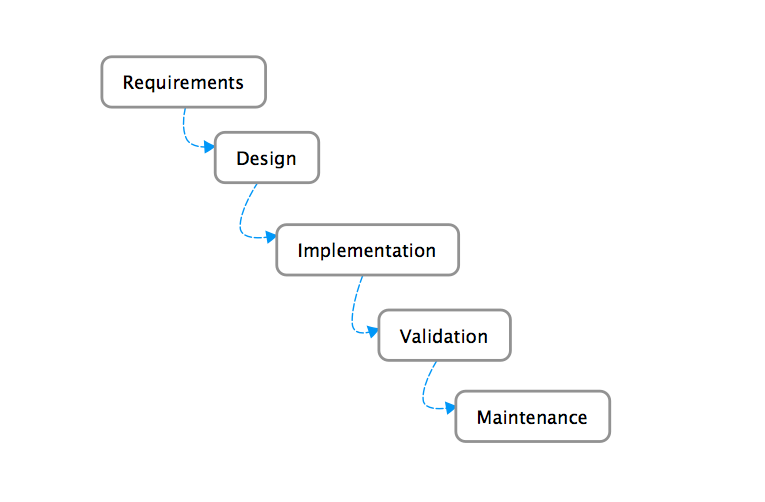
\includegraphics[width =0.8\linewidth]{WaterfallModel}}
\caption{The Waterfall Model}
\label{sec:WTF}
\label{fig:WTF}
\end{figure}

The Waterfall Model is a well documented process model, which has more simple approach and disciplined. The waterfall model provides a structured development approach. It includes:
\begin{enumerate}
	\item  Requirements
	\item  Design
	\item  Implementation (Coding or construction of the project)
	\item  Validation (Testing or debugging)
	\item  Maintenance
\end{enumerate}

\paragraph{Requirements}
At the Requirements specification phase, team will perform requirements elicitation based on the project description and the client meetings. All the selected requirements will be listed in the SRS document and implemented during the development phase.

\paragraph{Design:}
The Design phase is the phase that team members to design and establish a project plan. It is very important for the team to design all the aspects of the project.

\paragraph{Implementation:}
The main developers will start to implement the software of the project at this phase. Proper SRS documents and plans at earlier phases will be helpful. 

\paragraph{Validation:}
After the implementation is done, the QA engineers will start the Validation phase, involving testing the overall system and ensuring all requirements have being achieved. 

\paragraph{Maintenance:}
After the first release of the software, the team will need to maintain the system and fix possible bugs which would be found by users.

\subsection{Advantages}
\begin{enumerate}
	\item  Simple and disciplined linear software process flow.
	\item  Well written documentation will be produced earlier in the software life cycle.
	\item  Software release to the client on deadline.
\end{enumerate}

\subsection{Disadvantages}
\begin{enumerate}
	\item  Not flexible to changing.
	\item  Late discovery of technical problems.
	\item  Can not have working software until the end of the development.
	\item  No testing stage in the early phases.
\end{enumerate}

\subsection{Minimise the Negative Impact}


\chapter{Work plan}



\section{Work activities}



\section{Milestones}

\section{Schedule allocation}

\section{Resource allocation}

\pagebreak


\chapter{Supporting plans}

\section{Configuration management plan}

\section{Documentation plan}

\section{Quality assurance plan}

\pagebreak


% Appendicies %
\newpage
\appendix

\pagebreak

\chapter{}






\end{document}
